\documentclass[12pt,fleqn]{article}\usepackage{../common}
\begin{document}
Support Vector Machines

In their simplest form, SVMs are \textbf{linear classifiers} that do
\textbf{risk minimization}.

\begin{equation}
R(\Theta) \leq J(\Theta) = R_{emp}(\Theta) +
\sqrt{ \frac{h \times (log(\frac{2N}{h}) + 1) - log(\frac{\eta}{4})}{N}} \nonumber
\end{equation}
\textbf{h}: capacity of a clasifier \\
\textbf{N}: number of training points 

\begin{itemize}
   \item Vapnik and Chernovenkis proved that with probability $1-\eta$ previous
equation holds true.
\end{itemize}

\begin{itemize}
   \item Vapnik and Chernovenkis proved that with probability $1-\eta$ previous
equation holds true.
   \item SVM algorithm minimizes both $h$ and empirical risk at the same time by
   increasing seperation margin (less flexibility)
\end{itemize}

\begin{itemize}
   \item Vapnik and Chernovenkis proved that with probability $1-\eta$ previous
equation holds true.
   \item SVM algorithm minimizes both $h$ and empirical risk at the same time by
   increasing seperation margin (less flexibility)
   \item Let's derive the equations
\end{itemize}

Derivation

\begin{figure}[!hbp]
\center{
  \scalebox{1.0}{
  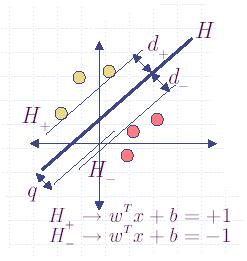
\includegraphics{svm-planes.png}
  }
}
\caption{}
\end{figure}

Decision plane: $w^{T}x + b=0$ \\
Let's define $q = min_{x}\big\|x - 0\big\|$

\begin{itemize}
   \item We will later use the formula for $q$ on $H^{+}$ and $H^{-}$.
   \item For H: $q = min_{x}\big\|x - 0\big\|$ subject to $w^{T}x+b=0$
   \item Lagrange: $min_{x}\frac{1}{2}\big\|x - 0\big\|^2+\lambda(w^{T}x+b)$
   \item Take gradient ($\frac{\partial}{\partial x}$) set to 0
   \item After some algebra: $q = \frac{|b|}{||w||}$
\end{itemize}


\begin{itemize}
  \item Define:
  \begin{itemize}  
  \item $H^{+} = w^{T}x + b=+1$
  \item $H^{-} = w^{T}x + b=-1$
  \end{itemize}
  \item This is without loss of generality; We can still adjust $b$ \& $w$
\end{itemize}

\begin{itemize}
  \item Calculate $q^{+}$ and $q^{-}$
  \begin{itemize}
  \item $q^{+} = \frac{|b-1|}{||w||}$
  \item $q^{-} = \frac{|-b-1|}{||w||}$
  \end{itemize}
  \item The margin then is 
  \begin{itemize}
  \item $m=q^{+}+q^{-} = \frac{|b-1-b-1|}{||w||} = \frac{|-2|}{||w||} = \frac{2}{||w||}$
  \end{itemize}  
\end{itemize}

For maximal margin, increase $m$ (maximize $\frac{2}{||w||}$) or minimize
$||w||$!

Constraints

We want points classified so that + and - points are in the correct side of the
hyperplanes;
\begin{eqnarray*}
w^{T}x+b \geq +1, \forall y_{i}=+1  \nonumber \\
w^{T}x+b \leq -1, \forall y_{i}=-1 \nonumber
\end{eqnarray*}
Combine the two
\begin{equation}
y_{i}(w^{T}x+b)-1 \geq 0 \nonumber
\end{equation}

Putting it all together

\begin{equation}
  min \frac{1}{2}{||w||^2} \textrm{ subject to }  y_{i}(w^Tx_{i}+b)-1 \ge 0 \nonumber
\end{equation}

This is a quadratic program!

qp

\begin{itemize}
   \item Python language has cvxopt package
   \item Matlab Optimization Toolbox has qp() function.
   \item Or Steve Gunn's SVM Toolbox has another qp written in C
   \item SVMLight has its own qp
   \item qp functions usually expect a problem in $\frac{1}{2}x^{T}Px+q^{T}x$
   format
   \item We can massage previous equation to fit the equation above
\end{itemize}


Dual

\begin{itemize}
   \item For SVM purposes, working with the dual  is easier.
   \item Form the Lagrange (again), take derivative, set equal to zero
   \item This gives us the KKT point
\end{itemize}

\begin{eqnarray}
L_{p} &=& \frac{1}{2}||w||^{2}-\sum_{i}\alpha_{i}(y_{i}(w^{T}x_{i}+b)-1)  \label{eq:primal}\\
\frac{\partial}{\partial w} L_{p} &=& w-\sum_{i}\alpha_{i}y_{i}x_{i}=0 \nonumber \\
w &=& \sum_{i}\alpha_{i}y_{i}x_{i} \label{eq:wdual} \\
\frac{\partial}{\partial b} L_{p} &=& -\sum_{i}\alpha_{i}y_{i}=0  \label{eq:cdual}
\end{eqnarray}

Plugging equation \ref{eq:wdual} and \ref{eq:cdual} into primal equation \ref{eq:primal}:
\begin{eqnarray}
\textrm{ Maximize } L_{D}=\sum_{i}\alpha_{i}-\frac{1}{2}\sum_{i}\sum_{j}\alpha_{i}\alpha_{j}y_{i}y_{j}x_{i}^{T}x_{j} \label{eq:svm}
\end{eqnarray}
constraints
\begin{eqnarray*}
\sum_{i}\alpha_{i}y_{i}=0 \nonumber \\
\alpha_{i} \geq 0 \nonumber
\end{eqnarray*}

qp

\begin{itemize}
   \item qp() again! But now the variable(s) we are solving for are
     $\alpha_i$'s, not $x$'s. 
   \item Massage \ref{eq:svm} into  $\frac{1}{2}x^{T}Px+q^{T}x$ form
   \item This can be achieved by setting $P_{i,j}$ to be $-y_{i}y_{j}x_{i}^{T}x_{j}$
   \item Call qp
   \item The solution is a list of $\alpha$'s 
\end{itemize}

Calculating $b$

\begin{itemize}
   \item Due to KKT condition, for each nonzero $\alpha_{i}$, the corresponding
   constraint in the primal problem is tight (an equality)
   \item Then for each non-zero $\alpha_{i}$, calculate $b$ using $w^{T}x_{i}+b = y_{i}$.
   \item Each $b$ from non-zero $\alpha_{i}$ will be approximately equal to
   other $b$'s. It is numerically safer to average all $b$'s for final $b$.
\end{itemize}

Classifier Done

For each new point $x$, we can use $sign(x^{T}w+b)$ as our classifier. The
result, $-1$ or $+1$ will tell us which class this new point belongs to.

Sample Output

\begin{figure}[!hbp]
\center{
  \scalebox{0.55}{
  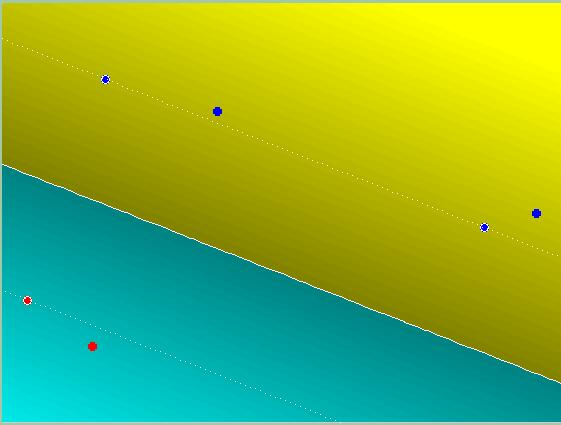
\includegraphics{svmlinear.png}
  }
}
\caption{}
\end{figure}

Kernels

\begin{itemize}
   \item We talked about linear boundaries so far
   \item SVMs can also form non-linear boundaries
   \item Simple: Just preprocess input data with a basis function into higher
   dimensions
   \item Rest of the algorithm is unchanged
\end{itemize}

Nonlinear Kernel


\begin{figure}[!hbp]
\center{
  \scalebox{0.55}{
  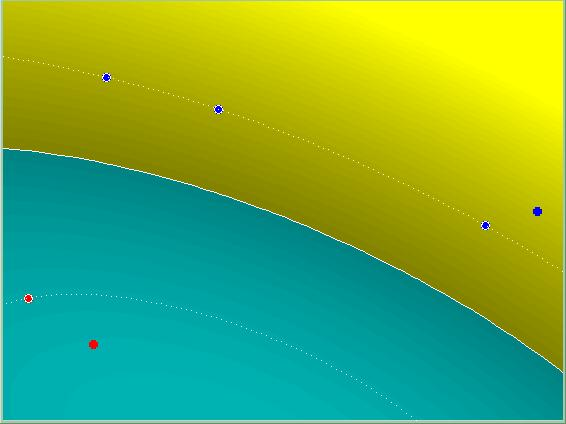
\includegraphics{svmpoly.png}
  }
}
\caption{}
\end{figure}

Slack

\begin{itemize}
   \item Sometimes the problem might be inseperable
   \item A few points might throw off the classifier
   \item We can introduce ``slack'' into a classifier
   \item For example, allow data to fall on the wrong side with $w^{T}+b \geq
   -0.03$ for $y_{i}=+1$
   \item But we don't want too many of such points, hence penalize the
   ``quantity'' of suck slack points
\end{itemize}

\clearpage

{\scriptsize
\begin{verbatim}
import numpy as np
from numpy import linalg
import cvxopt
import cvxopt.solvers

def svm(X, y):
    n_samples, n_features = X.shape

    # Gram matrix
    K = np.zeros((n_samples, n_samples))
    for i in range(n_samples):
        for j in range(n_samples):
            K[i,j] = np.dot(X[i], X[j])

    P = cvxopt.matrix(np.outer(y,y) * K)
    q = cvxopt.matrix(np.ones(n_samples) * -1)
    A = cvxopt.matrix(y, (1,n_samples))
    b = cvxopt.matrix(0.0)

    G = cvxopt.matrix(np.diag(np.ones(n_samples) * -1))
    h = cvxopt.matrix(np.zeros(n_samples))

    # solve QP problem
    solution = cvxopt.solvers.qp(P, q, G, h, A, b)

    print solution
    
    # Lagrange multipliers
    a = np.ravel(solution['x'])
    
    print "a", a

    # Support vectors have non zero lagrange multipliers
    ssv = a > 1e-5
    ind = np.arange(len(a))[ssv]
    a = a[ssv]
    sv = X[ssv]
    sv_y = y[ssv]
    print "%d support vectors out of %d points" % (len(a), n_samples)
    print "sv", sv
    print "sv_y", sv_y

    # Intercept
    b = 0
    for n in range(len(a)):
        b += sv_y[n]
        b -= np.sum(a * sv_y * K[ind[n],ssv])
    b /= len(a)
        
    # Weight vector
    w = np.zeros(n_features)
    for n in range(len(a)):
        w += a[n] * sv_y[n] * sv[n]

    print "a", a
    return w, b, sv_y, sv, a

if __name__ == "__main__":

    def test():
        X = np.array([[3.,3.],[4.,4.],[7.,7.],[8.,8.]])
        y = np.array([1.,1.,-1.,-1.])
        w, b, sv_y, sv, a = svm(X, y)
        print "w", w
        print "b", b
        print 'test points'
        print np.dot([2.,2.], w) + b # > 1
        print np.dot([9.,9.], w) + b # < -1
        
    test()
\end{verbatim}
}

Note: We are maximizing the dual $L_d$, but we are still calling the minimizer
\verb!qp()! function. Therefore the $q$'s, which represent the summation of all
$\alpha$'s are negated as seen above in \verb!np.ones(n_samples) * -1!. The
quadratic part already has the negated statement $-\frac{1}{2}$ in the
beginning, so the rest of does not have to change. 

References

http://www.mblondel.org/journal/2010/09/19/support-vector-machines-in-python

Jebara, T., Machine Learning Lecture, Columbia University


\end{document}
